\documentclass[12pt]{article}
\usepackage{amssymb}
\usepackage[UTF8]{ctex}
\usepackage{geometry}
\usepackage{units}
\usepackage{pifont}
\usepackage{bm}
\geometry{
	a4paper,
	total={150mm,240mm},
	left=30mm,
	top=27mm,
	}
\usepackage{amsmath}
\usepackage{enumerate}
\usepackage{lipsum}
\usepackage{graphicx}
\usepackage{hyperref}
\usepackage{indentfirst}
\usepackage[graphicx]{realboxes}
\usepackage{booktabs}
\usepackage{multicol}
\usepackage{multirow}
\usepackage{cases}
\usepackage{subfig}  
\usepackage{float}
\usepackage{pythonhighlight}
\usepackage{nicematrix}
\linespread{1.2}
\usepackage{hyperref}
\usepackage{abstract}
\usepackage{xcolor}
\usepackage[ruled]{algorithm2e}

\title{数字图象处理PJ:传统方法实现图像去雾}
\author{陈锐林 21307130148}
\date{\today}

\begin{document}
\bibliographystyle{plain}
\maketitle
\begin{Large}
\noindent 1.背景介绍:\par
\end{Large}
如果天空中有雾霾或者烟雾,我们拍摄的图片会变得模糊不清、对比度降低;不利于对信息的保存和后续的处理。图像去雾即通过一些算法,对图像进行处理,恢复模糊图片的细节和色彩。\\

\begin{large}
    \noindent 1.1.去雾任务难点概述:\par
\end{large}
现阶段去雾任务仍有很多难点。\par
从对雾的物理模型来说,需要较复杂的模型才能完成工作;并且很多时候这是一个不适定问题。\par
雾天拍摄的图效果差可能由光照、阴影、色彩很多问题造成;求解也复杂。\par
现实场景复杂,如白天和黑夜对同一场景的拍摄也存在很大区别。\par
有的场景下无法达到实时性去雾或对高分辨率的图,始终需要较长时间。\par
真实数据收集难,筛选标准高;合成数据集无法完美模拟现实场景。\\

\begin{large}
    \noindent 1.2.总结过去、现有方法:\par
\end{large}
首先是基于大气散射模型的算法。$\bm{I}(\bm{x})=\bm{D}(\bm{x})+\bm{A}(\bm{x})$,其中$\bm{I,D,A}$分别是观测到的图、经过衰减的无雾图、经过衰减的大气光。通过对衰减系数(透射率)的估算,即可恢复出无雾图;如暗通道先验\cite{2011Single}就是利用这一模型去估计透射率。在这篇文章之后,很多算法也都基于对透射率的修正和估算。\par
还有从图像增强的角度出发的算法。如对图像进行对比度拉伸、颜色变换、各种滤波;常见的方法有:直方图均衡化、Retinex增强、小波变换等等。\par
以及基于深度学习的去雾算法也崭露头角。深度学习的算法也大多希望通过估计一些系数来恢复图片,比如对单张图片进行估计的DehazeNet\cite{7539399},或者通过卷积采集多尺度特征的MSCNN\cite{2020Single},或者通过无监督学习学习参数的DAD\cite{Shao_2020_CVPR}。\par
总体上看,自从暗通道先验的做法提出之后,传统的方法大都聚焦在任何更好地估计透射率上;也很难做到巨大的突破。而基于深度学习的方法其本身的可解释性就比较差,再加上很多数据集也是人工合成的图片;可能会出现在合成数据集上所向披靡,但在真实世界中屡屡碰壁。所以这仍是一个很值得研究的话题。\\
\newpage
\begin{Large}
\noindent 2.选择算法介绍:\par
\end{Large}
本次实验,我实现了3种去雾算法;分别是Baseline--暗通道先验去雾算法\cite{2011Single}、基于图像增强的自动色彩均衡(ACE)算法\cite{ipol.2012.g-ace}、同样基于图像复原(大气散射模型)的全局去雾算\cite{Berman_2016_CVPR}法。\par
在接下来这部分,我会详细介绍这些算法的实现原理;并且进行一定的对比与联系。\\

\begin{large}
    \noindent 2.1.暗通道先验去雾(Baseline):\par
\end{large}
该算法基于大气散射模型:\begin{equation}\label{eqn-1} 
  \bm{I}(\bm{x}) = \bm{J}(\bm{x})t(\bm{x})+\bm{A}(1-t(\bm{x}))
\end{equation}
其中$\bm{I}$是有雾图像;$\bm{J}$是无雾图像;$\bm{A}$是大气光照值,$t$是该点的透射率;公式的左侧就能理解为考虑投射的环境衰减,右侧是环境光照。\par
该方法还需要定义图像的暗通道;其实就是在RGB三个通道中找到最小的值。再稍微考虑到图像的相邻像素间存在紧密联系;考虑将某点$\bm{x}=(a,b)$的暗通道值定义为以其为中心的正方形窗口某个三个通道中的最小值。定义如下:\begin{equation}\label{eqn-1} 
    J^{dark}(\bm{x}) = \mathop{\mathrm{min}}\limits_{\bm{y}\in \Omega({\bm{x}})}(\mathop{\mathrm{min}}\limits_{c\in\{r,g,b\}}J^{c}(\bm{x}))
\end{equation}
而该算法的重要的先验就是,在无雾图像$\bm{J}(\bm{x})$中,其暗通道$J^{dark}\rightarrow 0$。\par
回到对(1)的变形,单看某个通道$c$;变形为:\begin{equation}\label{eqn-1} 
  \frac{\bm{I}^c(\bm{x})}{\bm{A}^c} = t(\bm{x})\frac{\bm{J}^c(\bm{x})}{\bm{A}^c}+(1-t(\bm{x}))
\end{equation}再考虑窗口的影响,以及假定在较小的窗口内$t$是不变的,就有:
\begin{equation}\label{eqn-1} 
  \mathop{\mathrm{min}}\limits_{\bm{y}\in \Omega({\bm{x}})}(\mathop{\mathrm{min}}\limits_{c}\frac{\bm{I}^c(\bm{x})}{\bm{A}^c}) = \widetilde{t}(\bm{x}) \mathop{\mathrm{min}}\limits_{\bm{y}\in \Omega({\bm{x}})}(\mathop{\mathrm{min}}\limits_{c}\frac{\bm{J}^c(\bm{x})}{\bm{A}^c})+(1-\widetilde{t}(\bm{x}))
\end{equation}
而根据暗通道先验的条件,$\displaystyle\mathop{\mathrm{min}}\limits_{\bm{y}\in \Omega({\bm{x}})}(\mathop{\mathrm{min}}\limits_{c}\frac{\bm{J}^c(\bm{x})}{\bm{A}^c})\rightarrow 0$,于是只要得到$\widetilde{t}(\bm{x})$就可以复原出图片。\par
显然,这里的$\widetilde{t}(\bm{x})$就是:\begin{equation}\label{eqn-1} 
  \widetilde{t}(\bm{x}) = 1-\omega  \mathop{\mathrm{min}}\limits_{\bm{y}\in \Omega({\bm{x}})}(\mathop{\mathrm{min}}\limits_{c}\frac{\bm{I}^c(\bm{x})}{\bm{A}^c}) 
\end{equation}
其中,$\omega$是为了保留一部分的雾成分;会更真实。\par
在最终去雾前,对$t$进行一定的修正。这里采用的是导向滤波(因为比起soft matting效率高很多)。导向滤波的输入是目标图$P$(如我们这的$t(\bm{x})$)和引导图$I$(如我们的原图$\bm{I}(\bm{x})$,输出一张大体上与$P$相似,但是有着$I$纹理的图;能对我们得到的$t(\bm{x})$进行平滑和优化。具体计算如下:
\begin{figure}[h]
    \centering
    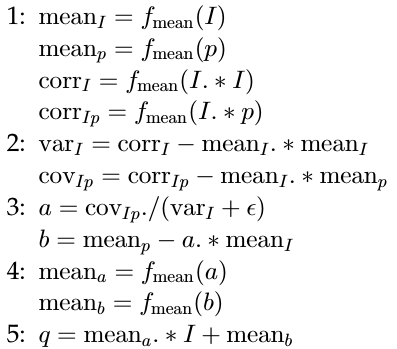
\includegraphics[width=0.4\textwidth]{dip4.jpg}
\end{figure}\\
这里的操作都只涉及元素乘($.*$和$./$),大部分功能由均值滤波实现。所以是在$O(N)$的复杂度。\par
于是最终图像恢复为:\begin{equation}\label{eqn-1} 
  \bm{J}(\bm{x})=\frac{\bm{I}(\bm{x})-\bm{A}}{\max(t(\bm{x}),t_0)}+\bm{A}
\end{equation}
为了避免因为$t(\bm{x})$过小导致结果太大,过于割裂。
\\

\begin{large}
    \noindent 2.2.自动色彩均衡(Automatic Color Enhancement ACE):\par
\end{large}
这个算法从图像增强的角度出发进行去雾;并不对场景做物理建模,而是直接对色调进行调整。根据原文可以看到,是仿照人视网膜的一些机制做的调整方案。\par
算法第一步是对每个通道值进行色差的校正。类似地,RGB三个通道分别处理,然后同样以点$\bm{x}=(a,b)$为中心作一个区域$\Omega$;利用邻近的信息对$\bm{x}$做恢复。具体计算如下:\begin{equation}\label{eqn-1} 
  \bm{R}(\bm{x})=\sum_{\bm{y}\in \Omega-\{\bm{x}\}}\frac{s_{\alpha}(\bm{I}(\bm{x})-\bm{I}(\bm{y}))}{\left\vert|\bm{x}-\bm{y}|\right\vert}
\end{equation}
其中$\bm{I}$是当前计算通道的值(就是计算了亮度差);距离采用欧氏距离,用来表示远近的权重;$s_{\alpha}$是一个映射函数,表达为$s_{\alpha}(t)=\min(1,\max(-1,\alpha t))$。这个函数控制我们的亮度范围,配合上之后的延展操作,可以做到压缩或者扩张范围的作用。其图示如下:
\begin{figure}[h]
    \centering
    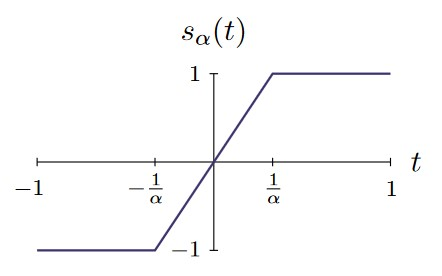
\includegraphics[width=0.4\textwidth]{dip1.jpg}
\end{figure}
\par
算法第二步是进行延申,这步主要是确保上面输出的$\bm{R}(\bm{x})$的上确界和下确界都达到1和0。具体公式如下:\begin{equation}\label{eqn-1} 
  \bm{L}(\bm{x})=\frac{\bm{R}(\bm{x})-\min R}{\max R-\min R}
\end{equation}
最后将图像重新乘回8bit的范围就可以了。\par
在这篇文献中,采用了卷积或者插值来降低复杂度。这个实现可能比较麻烦,而\cite{张方略2013自动色彩均衡算法的速度优化}提出了另一种快速的做法;其主要利用了两个假设:将图片做多次ACE和将图片进行尺寸缩放后做ACE并不会很大影响结果。\par
若基于以上假设,就能使用以下快速算法。主要思路在于缩小分辨率来加速计算。
\begin{algorithm}[htb]
\caption{FastACE($\bm{I},\alpha,\beta$)}
\LinesNumbered
\KwIn{待去雾图像$\bm{I}$,亮度函数中的$\alpha$,标识$\Omega$范围的$\beta$}
\KwOut{去雾图}
h,w = 图的长和宽\;
将$\bm{I}$\;resize为$\displaystyle(\frac{h + 1}{2},\frac{w + 1}{2})$,储存在$\bm{I'}$\;
递归求解HalfI = FastACE($\bm{I'},\alpha,\beta$)\;
将HalfI和$\bm{I'}$重新变回原来分辨率\;
最后输出结果:HalfI + ACE($\bm{I},\alpha,\beta$) - ACE($\bm{I'},\alpha,\beta$)\;
\end{algorithm}\\
这里其实就是通过降低分辨率先得到一个信息缺失的图;之后再通过原图进行一些信息的补充,即加上原图中各个信息的相关关系(因为前面的$\bm{R}$就是考察了周围信息得到的)再减掉当前元素的周围信息。\par
看起来,这并没有降低工作量,因为我们还在调用原来的ACE接口,然而原先的$\Omega$通常是一个很大的数,现在只需要设定为很小就可以了。(比如取300和3,就是意味指90000和9个点的区别)。
\\

\begin{large}
    \noindent 2.3.Non-Local Image Dehazing:\par
\end{large}
这个算法同样基于(1)中的大气散射模型和Baseline的暗通道先验;这里主要做的工作就是进一步完善$t(\bm{x})$的计算。\par
这个算法还有其余的先验条件。首先是一张图中不同的颜色数远小于总的像素数;所以可以把所有的像素根据某种规则分为一些簇类(这里取500个)。还可以判断,在清晰图像中归为一类的点,在有雾图中会形成一条线(haze-line),在这条线的两端就是原色$\bm{J}$和大气光$\bm{A}$。这点从下面这个图能很清晰地看到,并且在清晰图中距离近的(如紫色)在haze-line中一样离得近;而像红色部分就会分得更开。
\newpage
\begin{figure}[h]
    \centering
    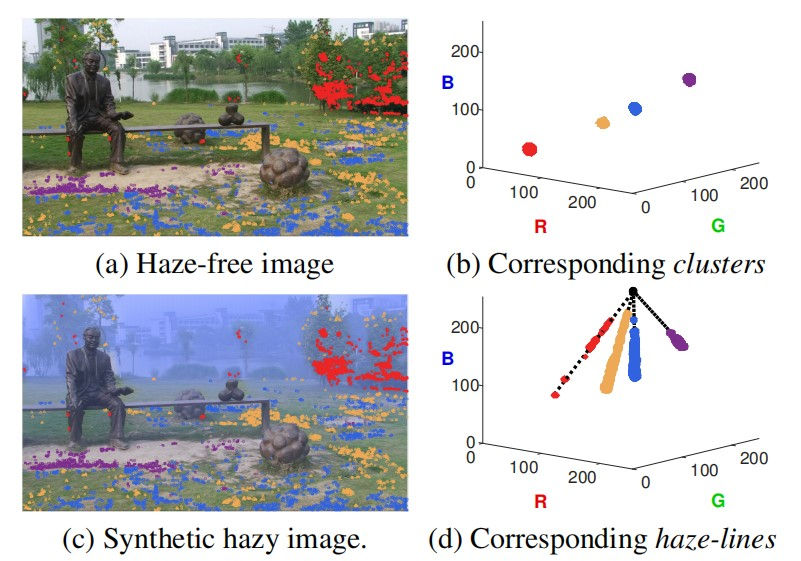
\includegraphics[width = 0.7\textwidth]{dip2.jpg}
\end{figure}
\par
算法第一步就是找到haze-line。取$\bm{I}_A=\bm{I}(\bm{x})-\bm{A}$为我们要寻找的;将其表示为$[r(\bm{x}), \theta(\bm{x}), \phi(\bm{x})]$。这里$r(\bm{x})$表示的距离,$\theta,\phi$用来标识其位置,可以理解为在上面这种RGB三个坐标中,已知$\bm{A}$,就还需要3个参数来找到当前的像素点。而利用公式(1)对$\bm{I}_A$进行变形,就可以得到$\bm{I}_A=  t(\bm{x}) · [\bm{J}(\bm{x}) − \bm{A}]$。考虑同一条线上的点,它们只有$t$是不同的,所以对于他们的$\theta,\phi$应该是一样的。那么我们如果我们作出一个球体来放置所有的像素点,每条haze-line上的点就处于同一个小方块,如下图。
\begin{figure}[h]
    \centering
    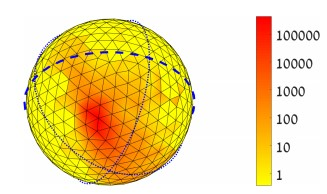
\includegraphics[width = 0.35\textwidth]{dip3.jpg}
\end{figure}\par
于是我们可以认为对两个共线的点,$\bm{J}_1 - \bm{A} = \alpha(\bm{J}_2-\bm{A})$,其中$\alpha$是一个比例。\par
在具体实现上,我们在对点进行分类时,就是用我们的$\theta,\phi$去和上面这个球表面的所有点比距离;簇类的实现使用KD-Tree实现即可,会比k-means快不少。\par
算法的第二步就是初步估计初始的透射率$t(\bm{x})$。根据前面的定义$\bm{r}(x)=t(\bm{x})\left\vert|\bm{J}-\bm{A}|\right\vert$,于是取透射率为1时的值为$r_{\max}$,那么$\displaystyle t(\bm{x})=\frac{r(\bm{x})}{r_{\max}}$。而针对每一簇haze-line,我们要找到最大的$\hat{r}_{\max}$,就只要遍历所有的点,找到$\displaystyle\max\limits_H\{r_{\max}\}$即可。\par
算法第三步是对$t(\bm{x})$做一些修正,原文的方法是利用类似于拉格朗日乘子去算;而我这直接复用了Baseline中的Guided Filter做修正。\par
算法第四步是完成图像复原的工作,和Baseline的做法一样,不再赘述。\\
\newpage
\begin{Large}
\noindent 3.实验介绍:\par
\end{Large}
本次实验对4个网络上的数据集:D-HAZY\cite{7532754}/HazeRD\cite{8296874}/O-HAZE\cite{O-HAZE_2018}/RESIDE\cite{li2019benchmarking},以及自己搜集的5张图片作了去雾的工作。\par
代码几乎都忠实地完成了算法的内容,除了个别地方修改(如将NonLocal的regularization改成GuidedFilter、并在Baseline和NonLocal最后都加了一个轻微的色调校正函数)。\par
对于所有图片都将其尺寸改到$600 \times 400$(长,宽);在一样的环境下运行了函数。最后记录了各个算法在每个数据集上的运行时间及各项指标,并且对实验结果进行了对比分析。\\

\begin{large}
    \noindent 3.1.实验启动:\par
\end{large}
项目内容已上传至Github,通过命令:\;git clone https://github.com/lrcc275/DIP-PJ.git 可以直接克隆。或者访问网址(\href{https://github.com/lrcc275/DIP-PJ.git}{point here})下载。\par
项目文件夹目录如下图。大部分的文件含义已经注明。较重点的是Report\_21307130148\_陈锐林.pdf是本次项目的报告;在代码中,evaluate.py是用来整个数据集跑的,需要手动修改里面的haze\_folder\_path和gt\_folder\_path,以及下面for循环中dehaze方法的选择,因为数据集的图片格式不一定相同,需要相应更改后面的通配符内容。main.py函数提供了一张图片的去雾(并展示),不过需要自己填上路径。
\begin{figure}[h]
    \centering
    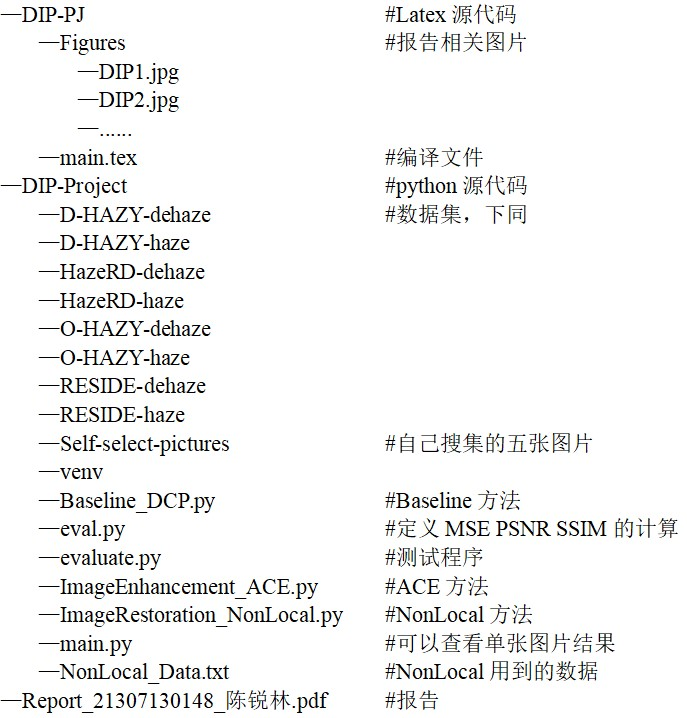
\includegraphics[width = 0.75\textwidth]{dip5.jpg}
\end{figure}
\newpage
\noindent 3.1.1.数据集介绍:\par
\begin{table}[h]
\centering
\begin{tabular}{ccccc} % 指定表格列数和对齐方式
\toprule 
数据集名 & 选用部分 & 图片对数  & 合成雾/真实雾 & 场景 \\ 
\midrule
D-HAZY & NYU\_GT  & 1449 & 合成 & 各种场景\\
HazeRD & all & 15(75张有雾选最模糊的) & 合成 & 室外\\
O-HAZE & all & 45 & 真实 & 室外 \\
RESIDE & SOTS & 542 & 合成 & 室外居多,少部分室内\\
\bottomrule 
\end{tabular}
\end{table}
此外还有自己收集的5张图片,后面会展示出来。\\

\noindent 3.1.2.实验设置介绍:\par
实验的基础设置就是将每张图片都转为$600\times 400$的大小,并且对每种算法、每个数据集进行测试;记录下各个指标即可。\par
在一些参数上,Baseline保留设定,即$r=7$的滤波半径、0.001\%的$\bm{A}$阈值、0.1的 $t_{\min} $。ACE中,$\alpha$设定为3,$r=4$的$\Omega$范围。在NonLocal中,暗通道的参数和Baseline一致。\\

\noindent 3.1.3.指标介绍:\par
主要就是用到三个指标$MSE,PSNR,SSIM$。\par
$MSE$是去雾图和数据集提供的清晰图之间,每个像素的平均差值。考虑到我们是彩色图像,所以$MSE$计算为:$\displaystyle \frac{1}{H\times W \times C}\sum_{i,j,c}(DI(i,j,c) - GT(i,j,c))^2$,这里$DI,GT$就是经过算法dehaze后的以及原始图。\par
$PSNR$是峰值信噪比,其表达式为$\displaystyle 10\log_{10}(\frac{(2^n-1)^2}{MSE})$。$n$为每像素的比特数,这里取8。\par
$SSIM$从亮度、对比度、结构三个方面衡量了图像间的相似性。我们先计算出两幅图像的均值、方差、协方差。分别记为:$\mu_x,\sigma_x,\mu_y,\sigma_y,\sigma_{xy}$。那么$SSIM$就等于:$$l(x,y)c(x,y)s(x,y)=\frac{2\mu_x\mu_y + c_1}{\mu_x^2+\mu_y^2+c_1}\;\frac{2\sigma_x\sigma_y + c_2}{\sigma^2_x + \sigma^2_y + c_2}\;\frac{\sigma_{xy}+c_3}{\sigma_x\sigma_y+c_3}$$
一般来说,三个常数分别取为$(0.01 \times 255)^2,(0.03 \times 255)^2,(0.01 \times 255)^2/2$。\par
$CIEDE2000$是一个重新定义了色差的指标。首先它将图片转为$L^*a^*b^*$空间(三个字母表示:亮度和两个对立维度)。它的计算如下:$$\displaystyle\Delta E = \sqrt{
(\frac{\Delta L}{K_L S_L})^2 + (\frac{\Delta C}{K_C S_C})^2 + (\frac{\Delta H}{K_H S_H})^2 + R_T(\frac{\Delta C}{K_C S_C})(\frac{\Delta H}{K_H S_H})
}$$
其中$\Delta L,\Delta H,\Delta C$分别是亮度差、色相差、色度差;$S_L,S_C,S_H$是三个由其他值计算出的权重信息;$K_L,K_C,K_H$是人工设置的因子;$R_T$是用于校正偏差的旋转因子。
\\

\begin{large}
    \noindent 3.2.实现方法在数据集上的各种指标结果:\par
\end{large}
首先是每个算法在各个数据集上的结果。
\begin{table}[h]
\centering
\begin{tabular}{ccccc} % 指定表格列数和对齐方式
\toprule 
\colorbox{yellow}{Baseline} & O-HAZE & RESIDE  & HazeRD & D-HAZY\\
\midrule
时间/s & 82.358 	& 815.400 & 26.024 	 & 2195.332  \\
$MSE$/img & 105.022  & 102.285 &  	99.141  &	102.647 \\
$PSNR$/img & 27.924 	&28.047 	&28.179 	&28.025 
 \\
$SSIM$/img & 0.654 	& 0.659 	&0.761 	&0.713 \\
$CIEDE2000$/img  & 30.873 	&28.114 &	17.380 &	32.234  
\\
\bottomrule 
\end{tabular}
\end{table}\par
\begin{table}[h]
\centering
\begin{tabular}{ccccc} % 指定表格列数和对齐方式
\toprule 
\colorbox{yellow}{ACE} & O-HAZE & RESIDE  & HazeRD & D-HAZY \\ 
\midrule
时间/s & 58.399 	&526.039 	&18.377 	&1429.121 
 \\
$MSE$/img & 105.068 	&106.178 	&104.331 	&105.204 
 \\
$PSNR$/img &27.924 	& 27.875 	&27.950 	&27.912 
 \\
$SSIM$/img & 0.668 	& 0.604 	& 0.778 	&0.674 
\\
$CIEDE2000$/img  &29.847 	&37.027 	&23.046 	&36.346 	\\
\bottomrule 
\end{tabular}
\end{table}\par
\begin{table}[h]
\centering
\begin{tabular}{ccccc} % 指定表格列数和对齐方式
\toprule 
\colorbox{yellow}{NonLocal} & O-HAZE & RESIDE  & HazeRD & D-HAZY \\ 
\midrule
时间/s & 62.654 	&550.781 	&22.630 	&1679.926 
  \\
$MSE$/img & 103.014 	&102.615 	&99.970 	&103.680 
 \\
$PSNR$/img & 28.007 	&28.032 	&28.136 	&27.981 
 \\
$SSIM$/img & 0.655 	&0.683 	&0.810 &	0.703 
\\
$CIEDE2000$/img  & 31.052 &	28.395& 	18.064 	&32.488 \\
\bottomrule 
\end{tabular}
\end{table}\par
以及每个算法的平均指标的对比。
\begin{table}[!h]
\centering
\begin{tabular}{cccc} % 指定表格列数和对齐方式
\toprule 
 & Baseline& ACE &NonLocal\\ 
\midrule
时间/s & 1.521	&0.991 	&1.129
  \\
$MSE$/img &102.577 	&105.452  &103.357 
 \\
$PSNR$/img  &28.030 	& 27.903 
&27.997 
 \\
$SSIM$/img & 0.698  &0.656	&0.697
\\
$CIEDE2000$/img & 31.007 & 36.286  & 31.270 \\
\bottomrule 
\end{tabular}
\end{table}\par
自己搜集的图像在下一部分展示。\\
\newpage
\begin{large}
    \noindent 3.3.样例介绍:\par
\end{large}首先展示我收集的5张有雾图像的去雾效果。\par
p1来自:\href{https://zhuanlan.zhihu.com/p/625819726}{【视觉影像】津门网江新华:雾景视界的美学观照.}
\begin{figure}[!h]
    \centering
    \begin{minipage}[t]{0.24\linewidth}
        \centering
        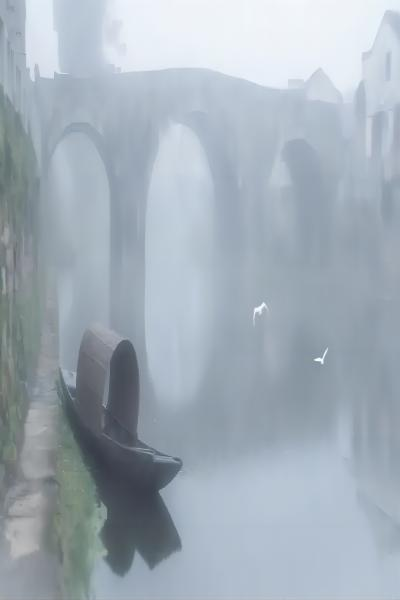
\includegraphics[width=0.9\linewidth]{sample_pictures/p1.jpg}
        \caption*{p1-原图}
    \end{minipage}
    \begin{minipage}[t]{0.24\linewidth}
        \centering
        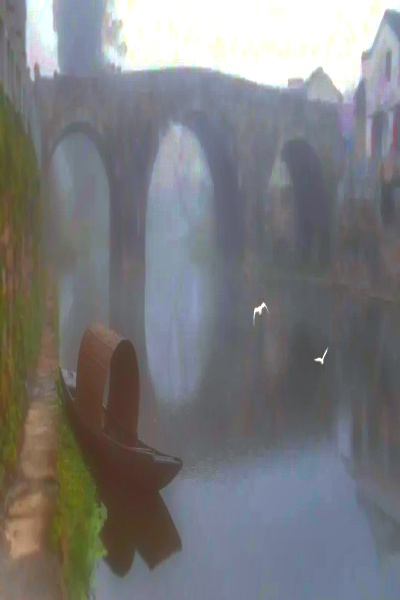
\includegraphics[width=0.9\linewidth]{sample_pictures/after_p1_Baseline.jpg}
        \caption*{p1-Baseline}
    \end{minipage}
    \begin{minipage}[t]{0.24\linewidth}
        \centering
        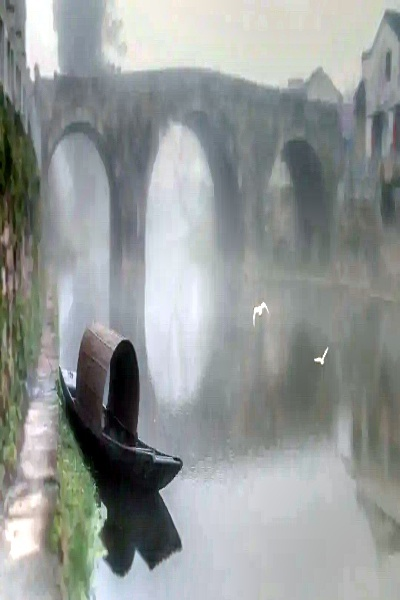
\includegraphics[width=0.9\linewidth]{sample_pictures/after_p1_ACE.jpg}
        \caption*{p1-ACE}
    \end{minipage}\begin{minipage}[t]{0.24\linewidth}
        \centering
        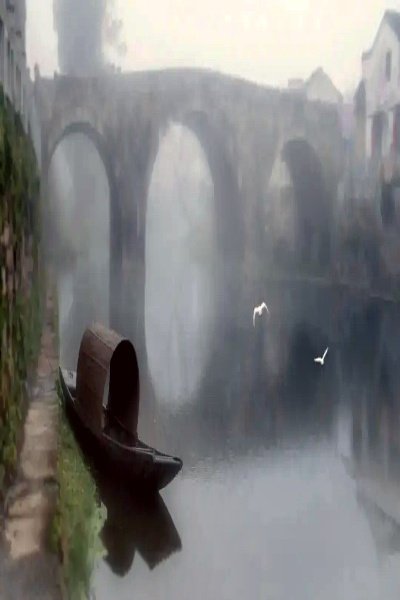
\includegraphics[width=0.9\linewidth]{sample_pictures/after_p1_NonLocal.jpg}
        \caption*{p1-NonLocal}
    \end{minipage}
 \end{figure}\par
 p2来自:\href{https://mbd.baidu.com/newspage/data/dtlandingsuper?nid=dt_4509732377873248581}{手机摄影|这不是油画 这是青岛今天的平流雾.}
 \begin{figure}[!h]
    \centering
    \begin{minipage}[t]{0.24\linewidth}
        \centering
        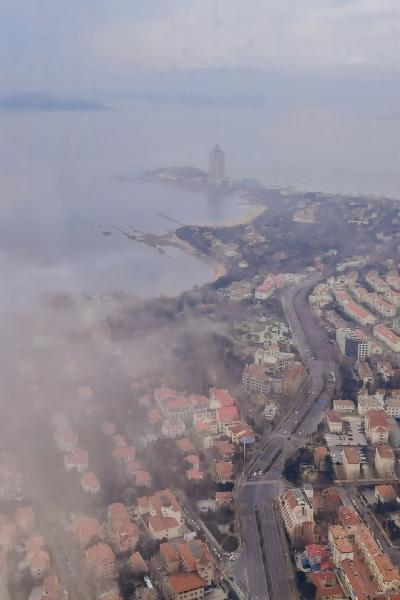
\includegraphics[width=0.9\linewidth]{sample_pictures/p2.jpg}
        \caption*{p2-原图}
    \end{minipage}
    \begin{minipage}[t]{0.24\linewidth}
        \centering
        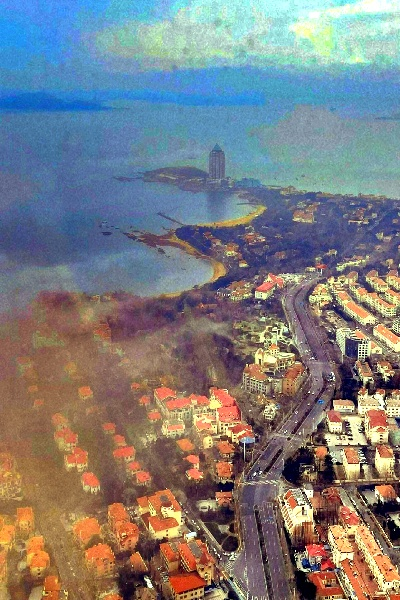
\includegraphics[width=0.9\linewidth]{sample_pictures/after_p2_Baseline.jpg}
        \caption*{p2-Baseline}
    \end{minipage}
    \begin{minipage}[t]{0.24\linewidth}
        \centering
        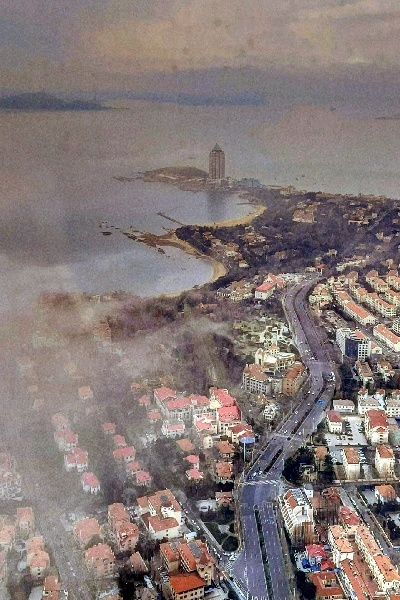
\includegraphics[width=0.9\linewidth]{sample_pictures/after_p2_ACE.jpg}
        \caption*{p2-ACE}
    \end{minipage}\begin{minipage}[t]{0.24\linewidth}
        \centering
        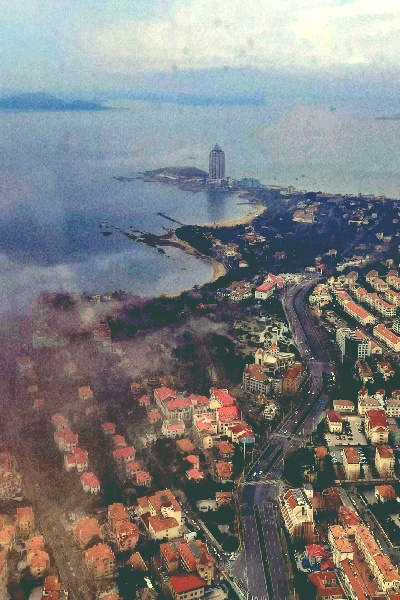
\includegraphics[width=0.9\linewidth]{sample_pictures/after_p2_NonLocal.jpg}
        \caption*{p2-NonLocal}
    \end{minipage}
 \end{figure}\par
 p3来自:\cite{2011Single}
 \begin{figure}[!h]
    \centering
    \begin{minipage}[t]{0.24\linewidth}
        \centering
        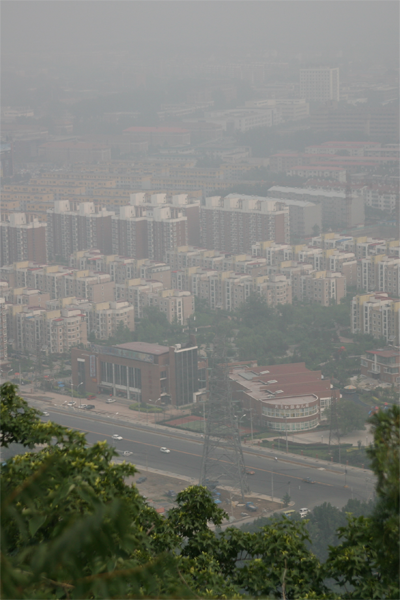
\includegraphics[width=0.9\linewidth]{sample_pictures/p3.jpg}
        \caption*{p3-原图}
    \end{minipage}
    \begin{minipage}[t]{0.24\linewidth}
        \centering
        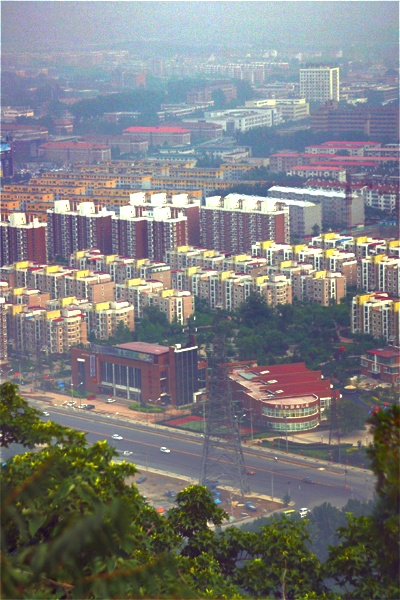
\includegraphics[width=0.9\linewidth]{sample_pictures/after_p3_Baseline.jpg}
        \caption*{p3-Baseline}
    \end{minipage}
    \begin{minipage}[t]{0.24\linewidth}
        \centering
        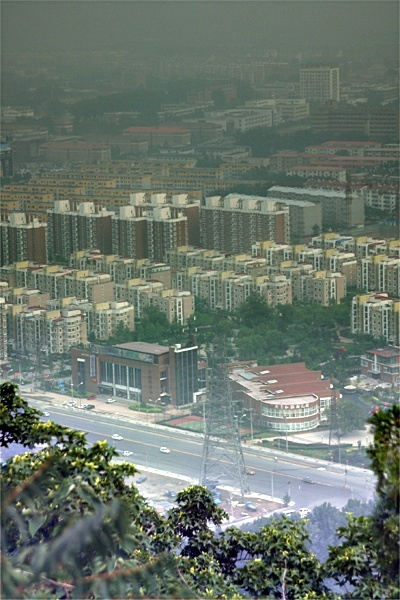
\includegraphics[width=0.9\linewidth]{sample_pictures/after_p3_ACE.jpg}
        \caption*{p3-ACE}
    \end{minipage}\begin{minipage}[t]{0.24\linewidth}
        \centering
        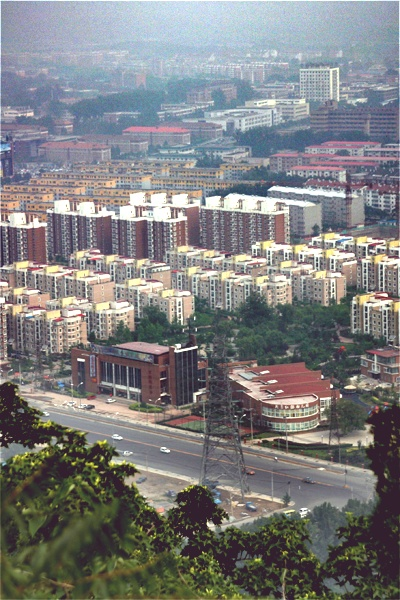
\includegraphics[width=0.9\linewidth]{sample_pictures/after_p3_NonLocal.jpg}
        \caption*{p3-NonLocal}
    \end{minipage}
 \end{figure}\par
 \newpage
 p4来自:\href{http://bbs.01ny.cn/forum.php?mod=viewthread&tid=3567038}{Adobe展示模拟“时光机”与超强除雾新技术}
 \begin{figure}[!h]
    \centering
    \begin{minipage}[t]{0.24\linewidth}
        \centering
        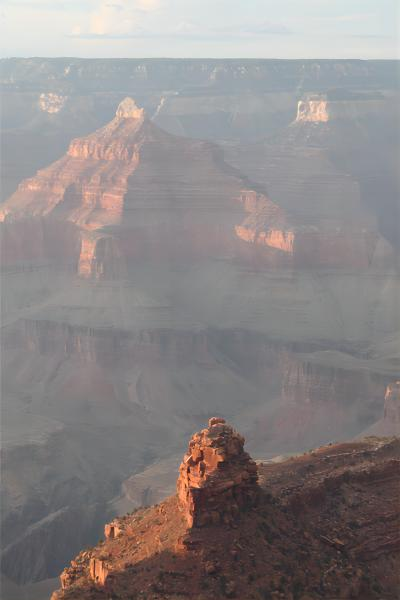
\includegraphics[width=0.9\linewidth]{sample_pictures/p4.jpg}
        \caption*{p4-原图}
    \end{minipage}
    \begin{minipage}[t]{0.24\linewidth}
        \centering
        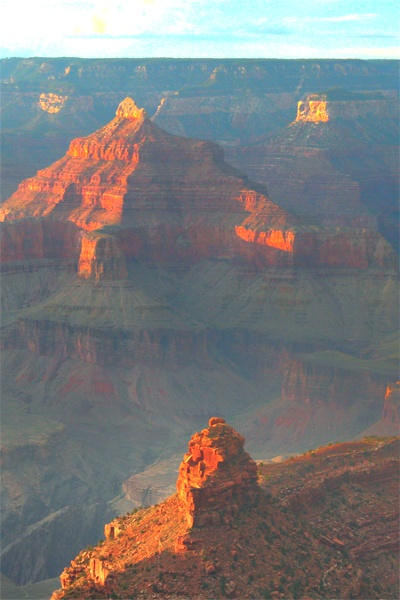
\includegraphics[width=0.9\linewidth]{sample_pictures/after_p4_Baseline.jpg}
        \caption*{p4-Baseline}
    \end{minipage}
    \begin{minipage}[t]{0.24\linewidth}
        \centering
        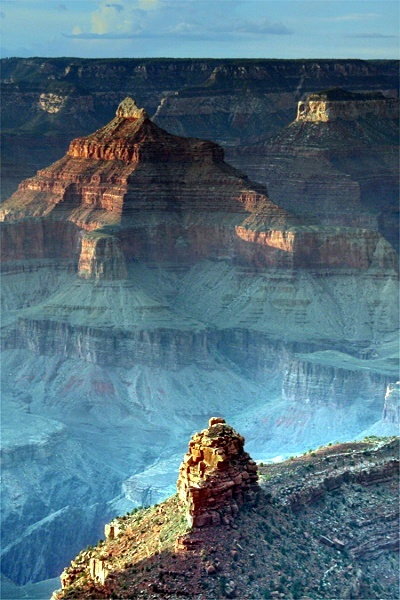
\includegraphics[width=0.9\linewidth]{sample_pictures/after_p4_ACE.jpg}
        \caption*{p4-ACE}
    \end{minipage}\begin{minipage}[t]{0.24\linewidth}
        \centering
        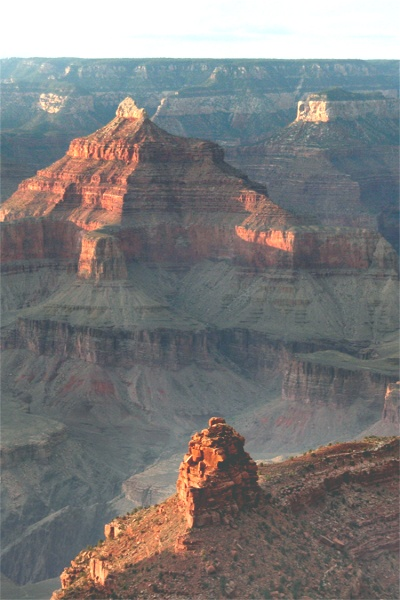
\includegraphics[width=0.9\linewidth]{sample_pictures/after_p4_NonLocal.jpg}
        \caption*{p4-NonLocal}
    \end{minipage}
 \end{figure}\par
 p5来自:\href{https://export.shobserver.com/baijiahao/html/572518.html}{上海现绝美平流雾,市民游客夜游宛如仙境的外滩.}
\begin{figure}[!h]
    \centering
    \begin{minipage}[t]{0.24\linewidth}
        \centering
        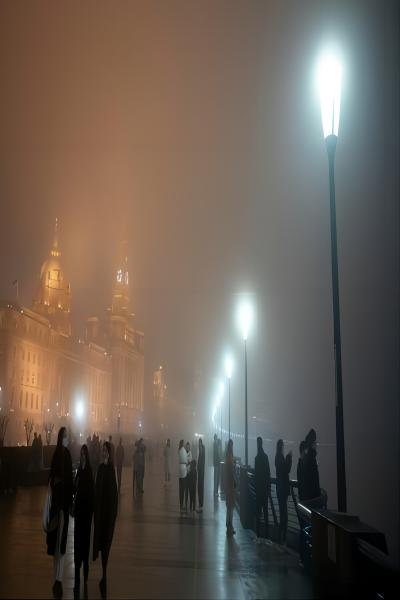
\includegraphics[width=0.9\linewidth]{sample_pictures/p5.jpg}
        \caption*{p5-原图}
    \end{minipage}
    \begin{minipage}[t]{0.24\linewidth}
        \centering
        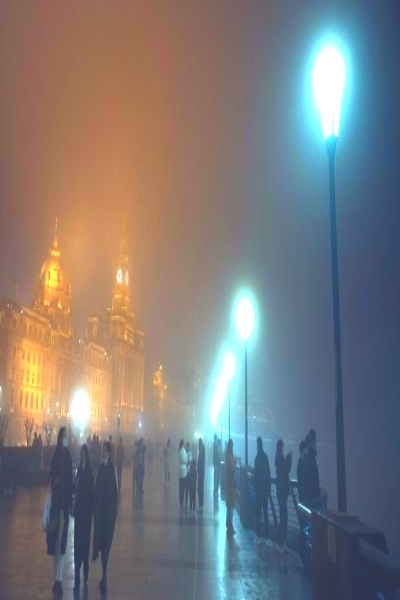
\includegraphics[width=0.9\linewidth]{sample_pictures/after_p5_Baseline.jpg}
        \caption*{p5-Baseline}
    \end{minipage}
    \begin{minipage}[t]{0.24\linewidth}
        \centering
        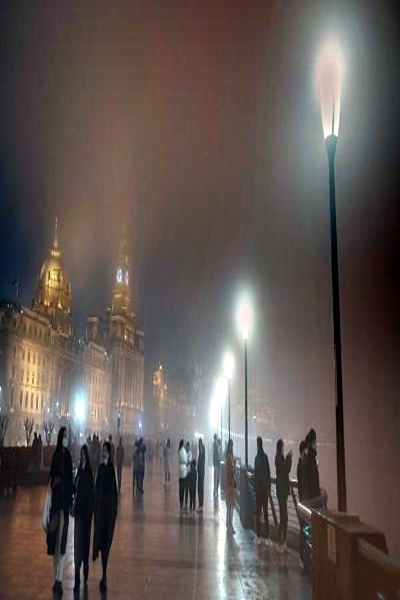
\includegraphics[width=0.9\linewidth]{sample_pictures/after_p5_ACE.jpg}
        \caption*{p5-ACE}
    \end{minipage}\begin{minipage}[t]{0.24\linewidth}
        \centering
        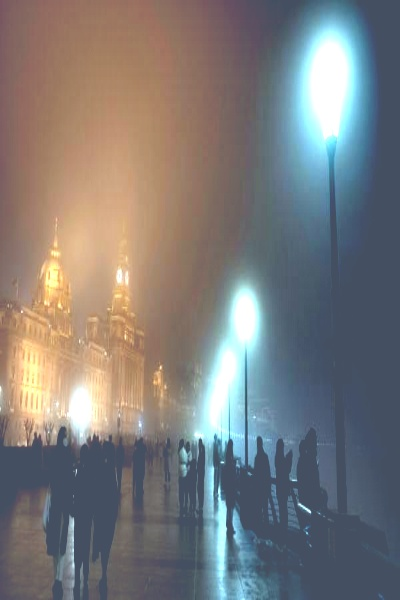
\includegraphics[width=0.9\linewidth]{sample_pictures/after_p5_NonLocal.jpg}
        \caption*{p5-NonLocal}
    \end{minipage}
 \end{figure}\par
 以及从各位数据集取的一张结果。\par
 从O-HAZY截取的:\begin{figure}[!h]
    \centering
    \begin{minipage}[t]{0.24\linewidth}
        \centering
        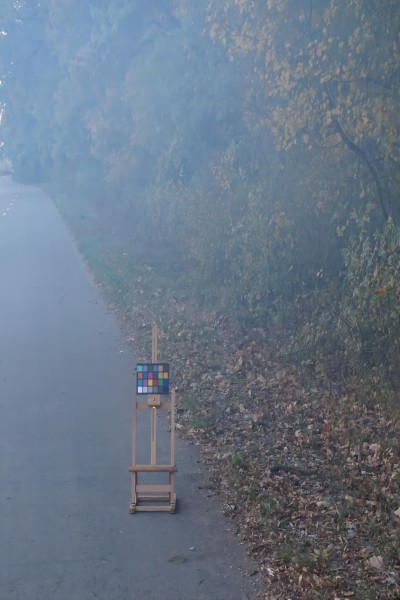
\includegraphics[width=0.9\linewidth]{sample_pictures/O-HAZY-example.jpg}
        \caption*{原图}
    \end{minipage}
    \begin{minipage}[t]{0.24\linewidth}
        \centering
        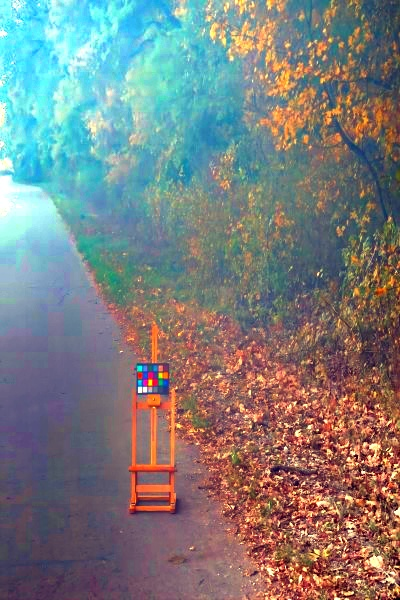
\includegraphics[width=0.9\linewidth]{sample_pictures/after_OHAZY_Baseline.jpg}
        \caption*{Baseline}
    \end{minipage}
    \begin{minipage}[t]{0.24\linewidth}
        \centering
        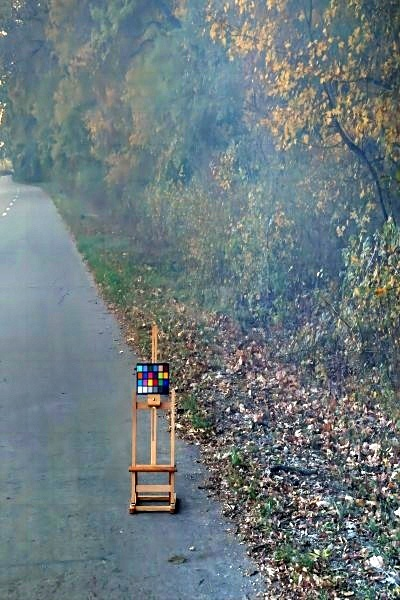
\includegraphics[width=0.9\linewidth]{sample_pictures/after_OHAZY_ACE.jpg}
        \caption*{ACE}
    \end{minipage}\begin{minipage}[t]{0.24\linewidth}
        \centering
        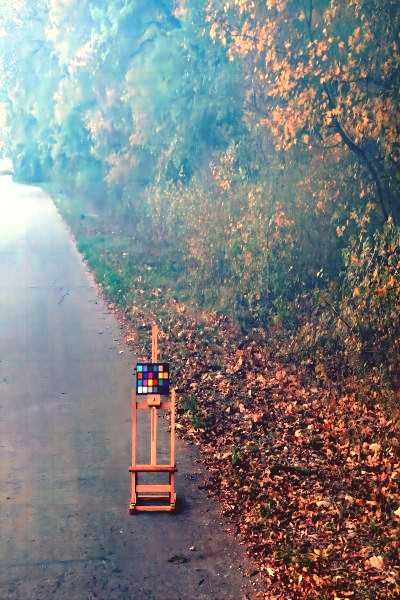
\includegraphics[width=0.9\linewidth]{sample_pictures/after_OHAZY_NonLocal.jpg}
        \caption*{NonLocal}
    \end{minipage}
 \end{figure}
 \newpage
 从HazeRD截取的:\begin{figure}[!h]
    \centering
    \begin{minipage}[t]{0.24\linewidth}
        \centering
        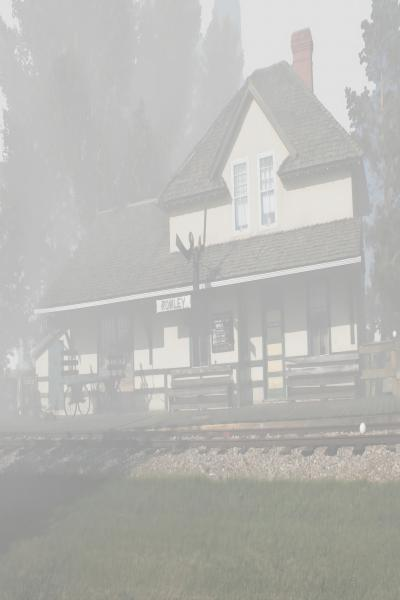
\includegraphics[width=0.9\linewidth]{sample_pictures/HazeRD-example.jpg}
        \caption*{原图}
    \end{minipage}
    \begin{minipage}[t]{0.24\linewidth}
        \centering
        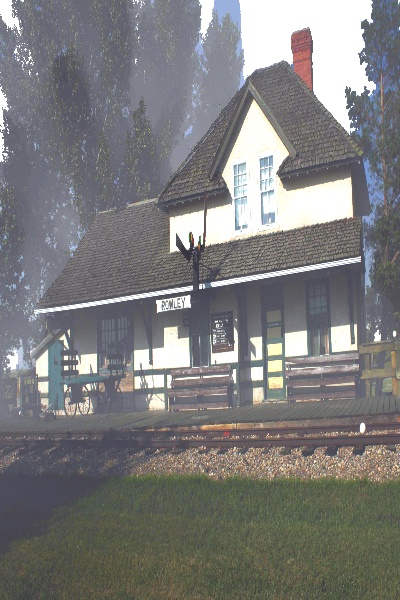
\includegraphics[width=0.9\linewidth]{sample_pictures/after_HazeRD_Baseline.jpg}
        \caption*{Baseline}
    \end{minipage}
    \begin{minipage}[t]{0.24\linewidth}
        \centering
        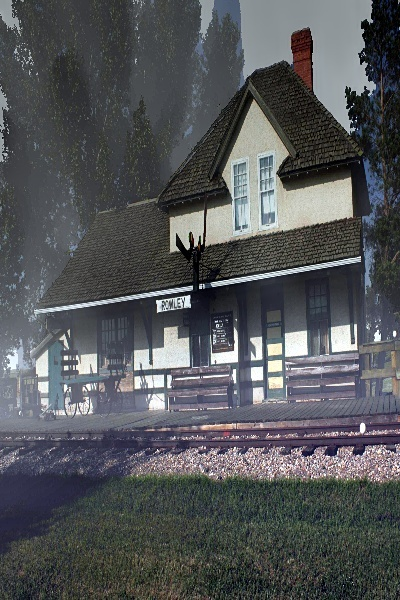
\includegraphics[width=0.9\linewidth]{sample_pictures/after_HazeRD_ACE.jpg}
        \caption*{ACE}
    \end{minipage}\begin{minipage}[t]{0.24\linewidth}
        \centering
        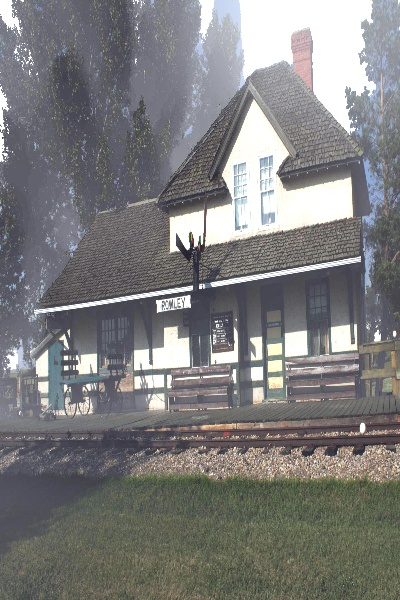
\includegraphics[width=0.9\linewidth]{sample_pictures/after_HazeRD_NonLocal.jpg}
        \caption*{NonLocal}
    \end{minipage}
 \end{figure}\par
 从D-HAZY截取的:\begin{figure}[!h]
    \centering
    \begin{minipage}[t]{0.24\linewidth}
        \centering
        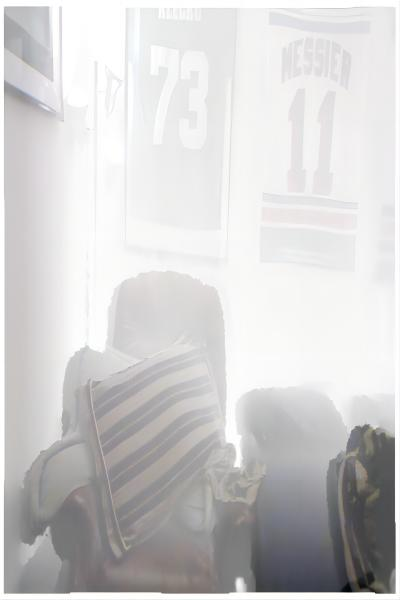
\includegraphics[width=0.9\linewidth]{sample_pictures/D-HAZY-example.jpg}
        \caption*{原图}
    \end{minipage}
    \begin{minipage}[t]{0.24\linewidth}
        \centering
        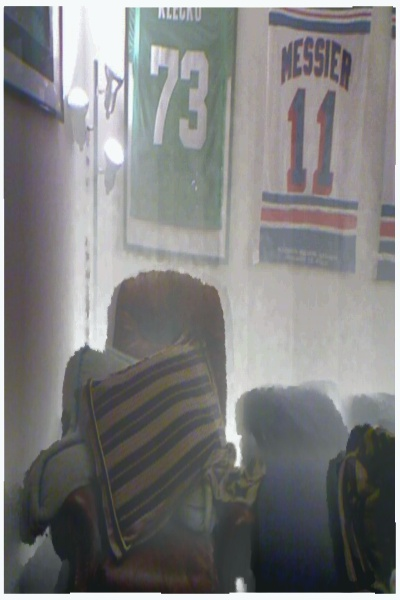
\includegraphics[width=0.9\linewidth]{sample_pictures/after_DHAZY_Baseline.jpg}
        \caption*{Baseline}
    \end{minipage}
    \begin{minipage}[t]{0.24\linewidth}
        \centering
        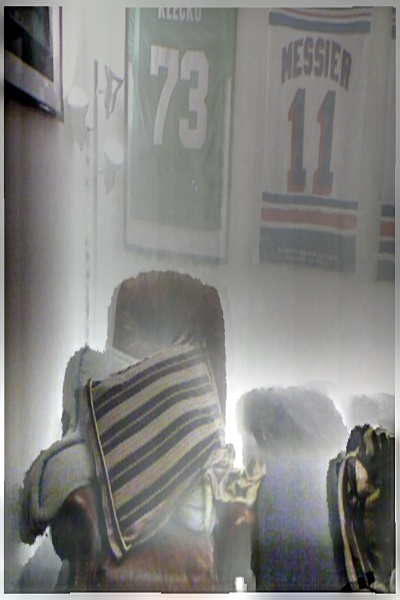
\includegraphics[width=0.9\linewidth]{sample_pictures/after_DHAZY_ACE.jpg}
        \caption*{ACE}
    \end{minipage}\begin{minipage}[t]{0.24\linewidth}
        \centering
        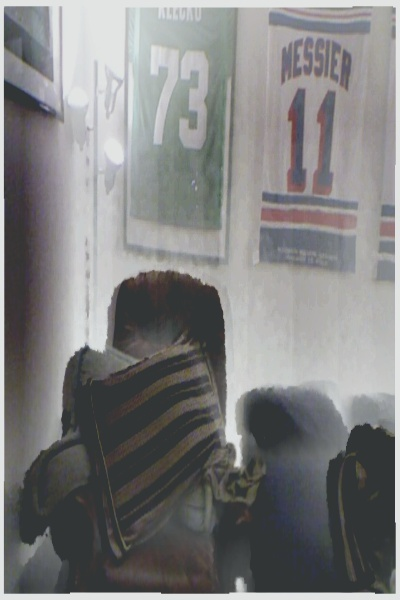
\includegraphics[width=0.9\linewidth]{sample_pictures/after_DHAZY_NonLocal.jpg}
        \caption*{NonLocal}
    \end{minipage}
 \end{figure}\par
 从RESIDE截取的:\begin{figure}[!h]
    \centering
    \begin{minipage}[t]{0.24\linewidth}
        \centering
        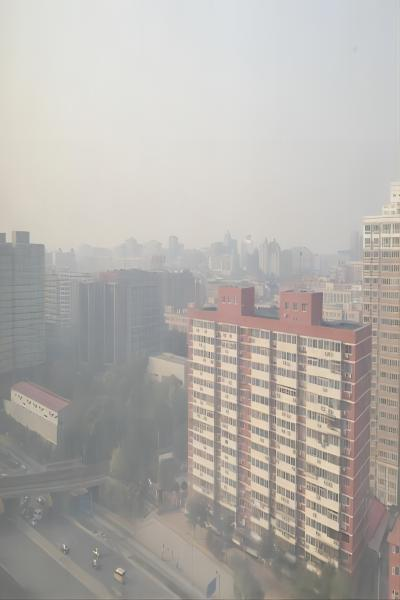
\includegraphics[width=0.9\linewidth]{sample_pictures/RESIDE-example.jpg}
        \caption*{原图}
    \end{minipage}
    \begin{minipage}[t]{0.24\linewidth}
        \centering
        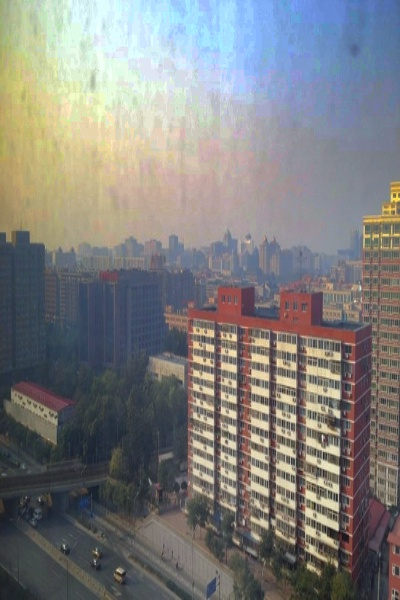
\includegraphics[width=0.9\linewidth]{sample_pictures/after_RESIDE_Baseline.jpg}
        \caption*{Baseline}
    \end{minipage}
    \begin{minipage}[t]{0.24\linewidth}
        \centering
        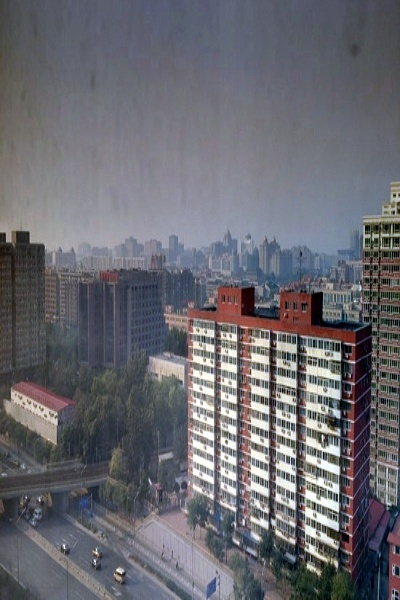
\includegraphics[width=0.9\linewidth]{sample_pictures/after_RESIDE_ACE.jpg}
        \caption*{ACE}
    \end{minipage}\begin{minipage}[t]{0.24\linewidth}
        \centering
        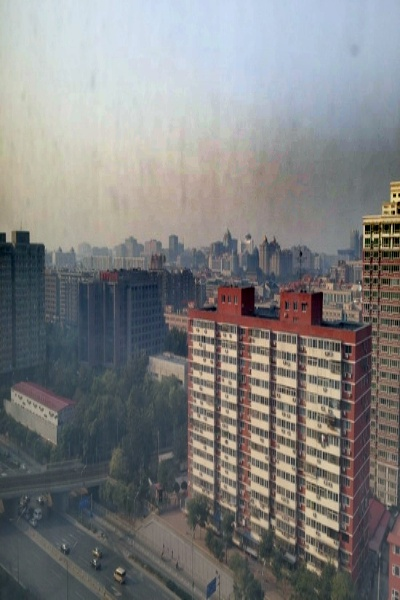
\includegraphics[width=0.9\linewidth]{sample_pictures/after_RESIDE_NonLocal.jpg}
        \caption*{NonLocal}
    \end{minipage}
 \end{figure}\par
需要注意的是因为Baseline和NonLocal方法直接生成会有点暗,所以这里是接了一个色彩的增强模块的(具体可以看代码),而ACE没有做(因为看着已经比较舒服了)。
\newpage
\begin{Large}
\noindent 4.结论与感悟:\par
\end{Large}
从本次实验的数据来看,Baseline算法的速度是较慢的;相比其和NonLocal的算法,透射率的求解是不同的。在Baseline中,是用腐蚀操作,对一个单元要考察范围是$15\times 15$的元素,就是$600 \times 400 \times 15 \times$;在NonLocal中是用kdtree来实现查找,查找的数据集是作者提供的一个1000个坐标的文件,所以对一个单元,进行查找的平均复杂度是$O(\log n)$,$n=1000$,即使opencv可能做出了相关的优化,NonLocal算法的开销还是小很多。同理,对ACE算法来说,首先它是递归求解的,真正求解是我们只要对周围的$3\times 3/ 4\times 4$的元素求解色差即可;这开销也是小的。\par
从其他指标结果来看,$MSE$和$PSNR$是差不多的,大概就是一个像素点有10的差距。而在$SSIM$和$CIEDE2000$上能较明显地看到暗通道的思想的优势。所以如果要选择一种适中的算法,兼具速度优势和效果优势的NonLocal会更好。\par
但是也必须说,指标的计算和人眼的测量差距还是很大的。如果对比着清晰图和经过算法去雾后的图,像上面O-HAZY那种,就会感觉Baseline的算法也太艳了点,ACE的还更接近现实,NonLocal比较适中;但是从指标上来看差距并不强烈;当然这里的“艳”是因为加了一个色彩校正,但不加的话反而暗得吓人,感觉更糟糕。\par
从未来的改进来说,如果还采用暗通道优先的方式,透射率的计算还是需要再改进;比如NonLocal中是有1000个预先提取的数据做KDtree的搜索,可以再多些点。并且NonLocal这种方法非常依赖于这些数据,选择更优的数据集是可行之策;并且如何在提高数据量的同时不让复杂度太大也是值得思考的。而ACE算法一个可行的方向是修改我们的$s_{\alpha}$函数的设计,可以采用其他符合要求的奇函数。\par
总的来说,在传统方法上,去雾工作仍然还有很大的改善空间。特别是在前几个数据集都鲜少有对夜间雾图的数据;因为夜间的情况也较复杂,可能非常雾和灯光(比如高层建筑物的光)是交杂在一起的,人眼能很好区分,但是计算机可能不行。
\\
\bibliography{ref}
\end{document}
